% Lecture file created by Gemini
% Class: Quantum Information With Atoms and Photons
% Professor: Pietro Silvi
% Date: 2025-10-16
\lecture{6}{Raman coupling}{2025-10-16}

% --- Start writing here ---
\section*{Raman Coupling: three-level atom}
\begin{center}
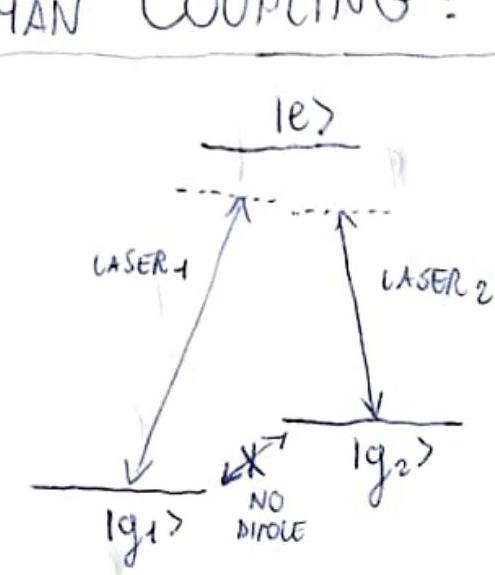
\includegraphics[max width=\textwidth]{2025_10_16_1968b45f52c890c3dc16g-1}
\end{center}

$$
\begin{aligned}
& H_{\text {ATOM }}=E_{1}\left|g_{1} \times g_{1} 1+E_{2}\right| g_{2} \times g_{2}\left|+E_{e}\right| e \times e \mid \\
& H_{\substack{\text { AIOM } \\
\text { I IGHT } \\
\text { INERAC. }}}=-\hat{\vec{d}} \cdot \hat{\vec{E}} \quad \text { WHERE }
\end{aligned}
$$

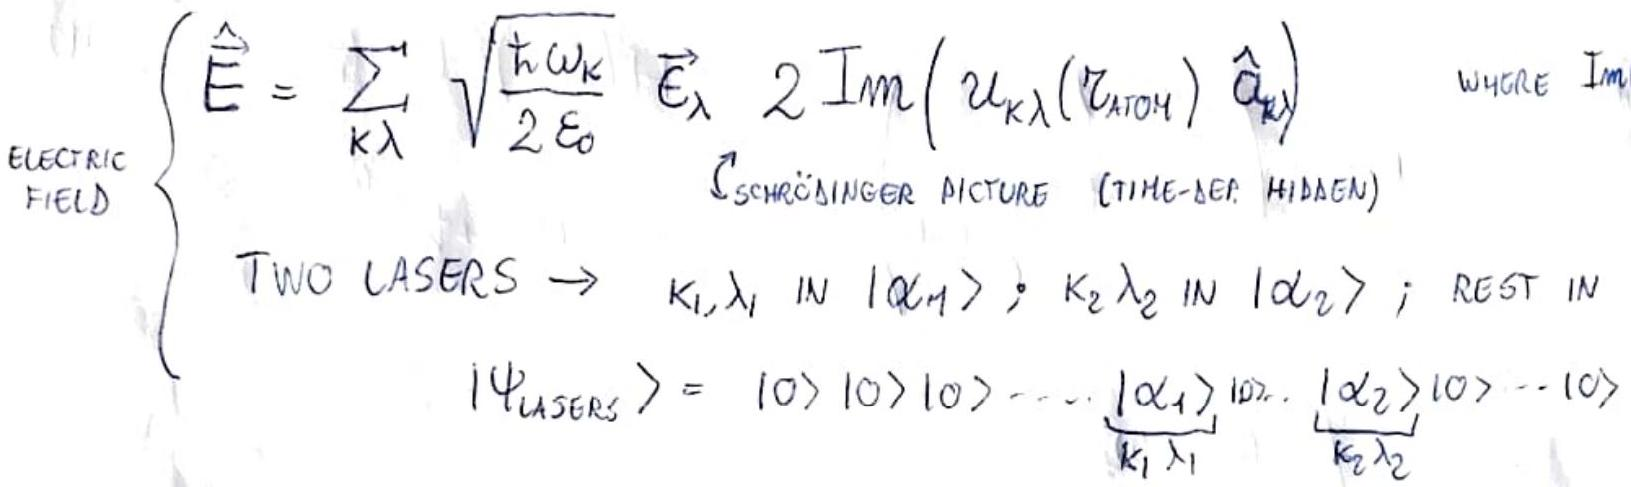
\includegraphics[max width=\textwidth, center]{2025_10_16_1968b45f52c890c3dc16g-1(1)}\\
$\left\langle\psi_{\text {LOCES }}\right| \vec{E}\left|\psi_{\text {LASERS }}\right\rangle=\sqrt{\frac{\hbar c K_{1}}{2 \varepsilon_{0}}} \vec{E}_{K_{1}} \lambda_{1} 2 \operatorname{Im}\left(u_{K_{1} \lambda_{i}}\left\langle\alpha_{1}\right| \alpha\left|\alpha_{1}\right\rangle e^{-i\left(c K_{1}\right) t}\right)+\binom{\text { SAME }}{K_{2} \lambda_{2}}$

$$
=\sqrt{\frac{2 \hbar c k_{1}}{\varepsilon_{0}}} \vec{\epsilon}_{x_{1} \lambda_{l}}|u|_{k_{1} \lambda_{1}}\left|\alpha_{1}\right| \cos \left(\left(c k_{1}\right) t+\phi_{1}\right)+\left(\operatorname{sAnt}_{k_{2}} \lambda_{2}\right.
$$

$\left(\begin{array}{l}\langle\vec{E}\rangle \text { OF TWO LASERS IS } \\ \text { OUST SON OE THE TWO } \\ \langle\vec{E}\rangle \text { FROM EACH LASER } \\ \text { (OPTICSI IS UNEAR) }\end{array}\right)$

$$
\langle\vec{E}\rangle=\vec{\xi}_{1} \cos \left(\omega_{1} t+\phi_{1}\right)+\vec{\xi}_{2} \cos \left(\omega_{2} t+\phi_{2}\right)
$$

$$
\begin{aligned}
& \underset{\substack{\text { INGH } \\
\text { INERACION }}}{H_{\text {ATOH }}}=-\left(\vec{d}_{\text {eg }}\left|e \times g_{1}\right|+\vec{d}_{\text {eg }}\left|e \times g_{2}\right|+\vec{d}_{\text {egl }}^{*}\left|g_{1} \times e\right|+\vec{d}_{\text {eg }}^{*}\left|g_{2} \times e\right|\right) \times \\
&\left(\vec{\varepsilon}_{1} \cos \left(\omega_{1} t+\phi_{1}\right)+\vec{\xi}_{2} \cos \left(\omega_{2} t+\phi_{2}\right)\right)= \\
& \Omega_{1}=\frac{\vec{d}_{\text {eg }}, \vec{\xi}_{1}}{\hbar} \quad \Omega_{2}=\frac{\vec{d}_{\text {eg }} \cdot \vec{\xi}_{2}}{\hbar} \quad \Omega_{1}=\frac{\vec{d}_{\text {eg }} \cdot \vec{\xi}_{2}}{\hbar} \quad \Omega_{2}=\frac{\vec{d}_{\text {eg }} \cdot \vec{\xi}_{1}}{\hbar}
\end{aligned}
$$

$$
\begin{aligned}
& H_{\text {ATOM-UGHT }}=-\hbar\left[\left|e \times g_{1}\right|\left(\Omega_{1} \cos \left(\omega_{1} t+\phi_{1}\right)+\Omega_{1} \cos \left(\omega_{2} t+\phi_{2}\right)\right)+\right. \\
& \left.\left|e \times g_{2}\right|\left(\Omega_{2} \cos \left(\omega_{2} t+\phi_{2}\right)+\mathscr{A}_{2} \cos \left(\omega_{1} t+\phi_{1}\right)\right)+\text { h.c. }\right] \\
& |g|\rangle \\
& |e\rangle \\
& \left|g_{2}\right\rangle \\
& H_{\text {FULL }}^{\binom{\text {LAE }}{\text { RAME }}}=-\hbar \\
& +\omega_{e g_{1}} \\
& \text { c.c. } \\
& \text { U } \\
& \text { c.c. } \\
& \Omega_{1} \omega s\left(\omega_{1} t+\phi_{1}\right)+X_{1} \omega s\left(\omega_{2} t+\phi_{2}\right) \\
& 0 \\
& \left.\Omega_{2}^{*} \cos \left(\omega_{2} t+\phi_{2}\right)+\mathscr{X}_{2} \cos \left(\omega_{1} t+\phi_{1}\right)+\omega_{e g_{2}}\right) \\
& \text { CIANGE GF } \\
& \text { REFERENCE } \\
& \text { FRAME } \\
& U(t)=\left(\begin{array}{cc}
e^{-i\left(\omega_{1} t+\phi_{1}\right)} & \\
& 1 \\
& e^{-i\left(\omega_{2} t+\phi_{2}\right)}
\end{array}\right) \\
& H\binom{\text { Ratai }}{\text { RRAME }}=U H\binom{\text { UAB }}{\text { FRAHE }} U^{+}+i \hbar \dot{U} U^{+} \\
& i \hbar \dot{U} U^{+}=+\hbar\left(\begin{array}{ccc}
\omega_{1} & & \\
& 0 & \\
& & \omega_{2}
\end{array}\right) \\
& H\left(\begin{array}{c}
\omega_{\text {eq },}-\omega_{1} \\
\Omega_{1} e^{i\left(\omega_{1} t+\phi_{1}\right)} \cos \left(\omega_{1} t+\phi_{1}\right)+\ldots
\end{array}\right. \\
& 0 \quad \Omega_{2}^{*} e^{-i\left(\omega_{2} t+\phi_{2}\right)} \cos \left(\omega_{i} t+\phi_{2}\right)+\ldots \omega_{e g_{2}}-\omega_{2} \\
& \delta_{1}=\omega_{e g_{1}}-\omega_{1} \quad \delta_{2}=\omega_{e g_{2}}-\omega_{2} ; H(t)=H_{0}+V(t) \\
& H_{0}=-\hbar\left(\begin{array}{ccc}
\delta_{1} & \Omega_{1}^{*} / 2 & 0 \\
\Omega_{1} / 2 & 0 & \Omega_{2} / 2 \\
0 & \Omega_{2}^{*} / 2 & \delta_{2}
\end{array}\right) \\
& V(t)=-\hbar\left(\begin{array}{ccc}
0 & c c . & 0 \\
\frac{\Omega_{1}}{2} e^{i\left(\omega_{1} t+\phi_{1}\right)}+\frac{{\mu_{i}}_{2}}{2} e^{i\left(\omega_{1}+\omega_{2}\right) t} e^{i \phi_{1}+\phi_{2}}+\frac{{\alpha_{1}}^{2} e^{i\left(\omega_{1}-\omega_{2}\right) t} e^{\left.i \phi_{1}-\phi_{2}\right)}}{0} & c . c . \\
0 & \begin{array}{l}
\text { SOMETH ING } \\
\text { SIM } \omega R
\end{array} & 0
\end{array}\right)
\end{aligned}
$$

$$
H_{\text {eff }} \simeq H_{0}+\frac{1}{\hat{\omega}}\left[V, V^{+}\right]+O\left(\frac{1}{\hat{\omega}^{2}}\right)
$$

\section*{RWA?}
$\tau$ osciustion frequencies of $V(t)$\\
$\frac{1}{\tilde{\omega}}\left[V, V^{+}\right]$is negligible wien Ho-timescales $\gg \frac{1}{\tilde{\omega}}$

BASICALLY or $H_{0}$-energyscales $\ll \hbar \tilde{\omega}$

$$
\Omega_{1}, \Omega_{2},\left|\delta_{1}\right|,\left|\delta_{2}\right| \ll \omega_{1}, \omega_{2},\left|\omega_{1}-\omega_{2}\right|
$$

RWA! $A_{N D} A S O A_{1} D_{2}$

AND NOW\\
$H_{\text {eff }}=H_{0}=\hbar\left(\begin{array}{ccc}+\left|\frac{\Omega_{1}}{2}\right| & \delta_{1} & \left|\frac{\Omega_{2}}{2}\right| \\ 0 & \left|\frac{\Omega_{2}}{2}\right| & \Delta=\delta_{1}-\delta_{2}\end{array}\right. t_{\text {and }}$ V\\
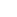
\includegraphics[width=0.5\textwidth, center]{2025_10_16_1968b45f52c890c3dc16g-3}\\
the two lasers can not BE TOO Close IN $\omega$

ALMOST LIKE THE 3-level problem we SOWES EARUER IN THE COURSE\\
let's say\\
|g. (e) $\quad g_{2}$ )\\
$H_{\text {UNP }}=\left(\begin{array}{ccc}0 & & \\ & \hbar \delta_{1} a \hbar \delta_{2} & \\ & & 0\end{array}\right) \quad H_{\text {PERT }}^{(A)}=\left(\begin{array}{cc}0 & \Omega_{1} \\ \Omega_{1} & 0 \\ \Omega_{2} & \Omega_{2}\end{array}\right) \frac{\hbar}{2} \quad H_{\text {Pecr }}^{(B)}=\left(\begin{array}{cc}0 & \\ 0 & \\ & \hbar \Delta\end{array}\right)$\\
perturbation theory on $\left\{\left|g_{1}\right\rangle,\left|g_{2}\right\rangle\right\}$ Itoraer\\
$\begin{array}{ll}\hat{\imath} & \\ \text { I CRAER } & \text { (EXACT Do) }\end{array}$\\
$H_{A}^{(2)}=\pi_{0} H^{(A)} R_{0} H^{(3)} \Pi_{0}=\hbar\left(\begin{array}{cc}1 & \\ & 0 \\ & \\ & 1\end{array}\right)\left(\begin{array}{ccc}0 & & \\ \Omega_{1} & 0 & \\ & \Omega_{2} & 0\end{array}\right)\left(\begin{array}{ccc}0 & & \\ & -1 / \delta & \\ & & 0\end{array}\right)\left(\begin{array}{ccc}0 & & \Omega_{1} \\ \Omega_{1} & 0 & \\ & \Omega_{2} & \\ & & \\ & & \end{array}\right)\left(\begin{array}{lll}1 & & \\ & 0 & \\ & & 1\end{array}\right)$\\
$H_{\text {FINAL }}^{\substack{\text { (Rot prime } \\ \text { FFRALE }}}=-\frac{\hbar}{4 \delta}\left(\begin{array}{cc}\Omega_{1}^{2} & \Omega_{1} \Omega_{2} \\ \Omega_{1} \Omega_{2} & \Omega_{2}^{2}\end{array}\right)+\hbar\left(\begin{array}{cc}0 & 0 \\ 0 & \Delta\end{array}\right)$\\
$=\hbar\left(-\frac{\Omega_{1} \Omega_{2}}{4 \delta}\right) \sigma^{x}+\hbar\left(\frac{\Omega_{2}^{2}-\Omega_{1}^{2}}{8 \delta}-\Delta\right) \sigma^{z}+$ const.
